%%%%%%%%%%%%%%%%%%%%%%%%%%%%%%%%%%%%%%%%%
% Short Sectioned Assignment
% LaTeX Template
% Version 1.0 (5/5/12)
%
% This template has been downloaded from:
% http://www.LaTeXTemplates.com
%
% Original author:
% Frits Wenneker (http://www.howtotex.com)
%
% License:
% CC BY-NC-SA 3.0 (http://creativecommons.org/licenses/by-nc-sa/3.0/)
%
%%%%%%%%%%%%%%%%%%%%%%%%%%%%%%%%%%%%%%%%%

%----------------------------------------------------------------------------------------
%	PACKAGES AND OTHER DOCUMENT CONFIGURATIONS
%----------------------------------------------------------------------------------------

\documentclass[paper=a4, fontsize=11pt]{scrartcl} % A4 paper and 11pt font size

\usepackage[T1]{fontenc} % Use 8-bit encoding that has 256 glyphs
\usepackage{fourier} % Use the Adobe Utopia font for the document - comment this line to return to the LaTeX default
\usepackage[english]{babel} % English language/hyphenation
\usepackage{amsmath,amsfonts,amsthm} % Math packages
\usepackage{float}
\usepackage{lipsum} % Used for inserting dummy 'Lorem ipsum' text into the template
\usepackage{graphicx}
\usepackage{sectsty} % Allows customizing section commands
\allsectionsfont{ \normalfont\scshape} % Make all sections centered, the default font and small caps

\usepackage{fancyhdr} % Custom headers and footers
\pagestyle{fancyplain} % Makes all pages in the document conform to the custom headers and footers
\fancyhead{} % No page header - if you want one, create it in the same way as the footers below
\fancyfoot[L]{} % Empty left footer
\fancyfoot[C]{} % Empty center footer
\fancyfoot[R]{\thepage} % Page numbering for right footer
\renewcommand{\headrulewidth}{0pt} % Remove header underlines
\renewcommand{\footrulewidth}{0pt} % Remove footer underlines
\setlength{\headheight}{13.6pt} % Customize the height of the header

\numberwithin{equation}{section} % Number equations within sections (i.e. 1.1, 1.2, 2.1, 2.2 instead of 1, 2, 3, 4)
\numberwithin{figure}{section} % Number figures within sections (i.e. 1.1, 1.2, 2.1, 2.2 instead of 1, 2, 3, 4)
\numberwithin{table}{section} % Number tables within sections (i.e. 1.1, 1.2, 2.1, 2.2 instead of 1, 2, 3, 4)

\setlength\parindent{0pt} % Removes all indentation from paragraphs - comment this line for an assignment with lots of text

%------------------------
% 	CODE RELATED PACKAGES
%------------------------
\usepackage{listings}

\usepackage[usenames,dvipsnames]{color} % Required for custom colors

\definecolor{dkgreen}{rgb}{0,0.6,0}
\definecolor{gray}{rgb}{0.5,0.5,0.5}
\definecolor{mauve}{rgb}{0.58,0,0.82}

\lstset{frame=tb,
  language=Java,
  aboveskip=3mm,
  belowskip=3mm,
  showstringspaces=false,
  columns=flexible,
  basicstyle={\small\ttfamily},
  numbers=none,
  numberstyle=\tiny\color{gray},
  keywordstyle=\color{red},
  commentstyle=\color{dkgreen},
  stringstyle=\color{mauve},
  breaklines=true,
  breakatwhitespace=true,
  tabsize=1,
        numbers=left, % Line numbers on left
        firstnumber=1, % Line numbers start with line 1
        numberstyle=\tiny\color{Blue}, % Line numbers are blue and small
        stepnumber=2 % Line numbers go in steps of 5
}


\newcommand{\java}[2]{
\begin{itemize}
\item[]\lstinputlisting[caption=#2,label=#1]{#1}
\end{itemize}
}


% \newcommand{\javalines}[2]{
% \begin{itemize}
% \item[]\lstinputlisting[caption=#2,label=#1, firstline=#3, lastline=#4]{#1}
% \end{itemize}
% }

%----------------------------------------------------------------------------------------
%	TITLE SECTION
%----------------------------------------------------------------------------------------

\newcommand{\horrule}[1]{\rule{\linewidth}{#1}} % Create horizontal rule command with 1 argument of height

\title{	
\normalfont \normalsize 
\textsc{IT University of Copenhagen} \\ [25pt] % Your university, school and/or department name(s)
\horrule{0.5pt} \\[0.4cm] % Thin top horizontal rule
\huge Model Driven Development Project \\ % The assignment title
\large A Configurator Project \\ % The subtitle
\horrule{2pt} \\[0.5cm] % Thick bottom horizontal rule
}


\author{
  Jorgensen, Anders B.\\
  \texttt{abrj}
  \and
  Helvind, Jakob B.\\
  \texttt{jbah}
  \and
  Hartvig, Martin R.\\
  \texttt{mrha}
  \and
  Kjerri, Rune M.\\
  \texttt{rmkj}
}
\date{\normalsize\today} % Today's date or a custom date

\begin{document}

\maketitle % Print the title
\newpage
%--------- START -------------------------------------------------------------------------------


% 2. An Example textual model in your DSL (in concrete syntax). No commentary is expected.
\section{An Example textual model}
\java{../configproject/runtime-CarFactory/src/factory.smdpdsl}{Concrete syntax of a CarFactory}

% 3. The Meta-model of your language (abstract syntax). Consider using several views, to improve presentation. No commentary is expected.
\section{The Meta-model}
\begin{figure}[H]
\centering
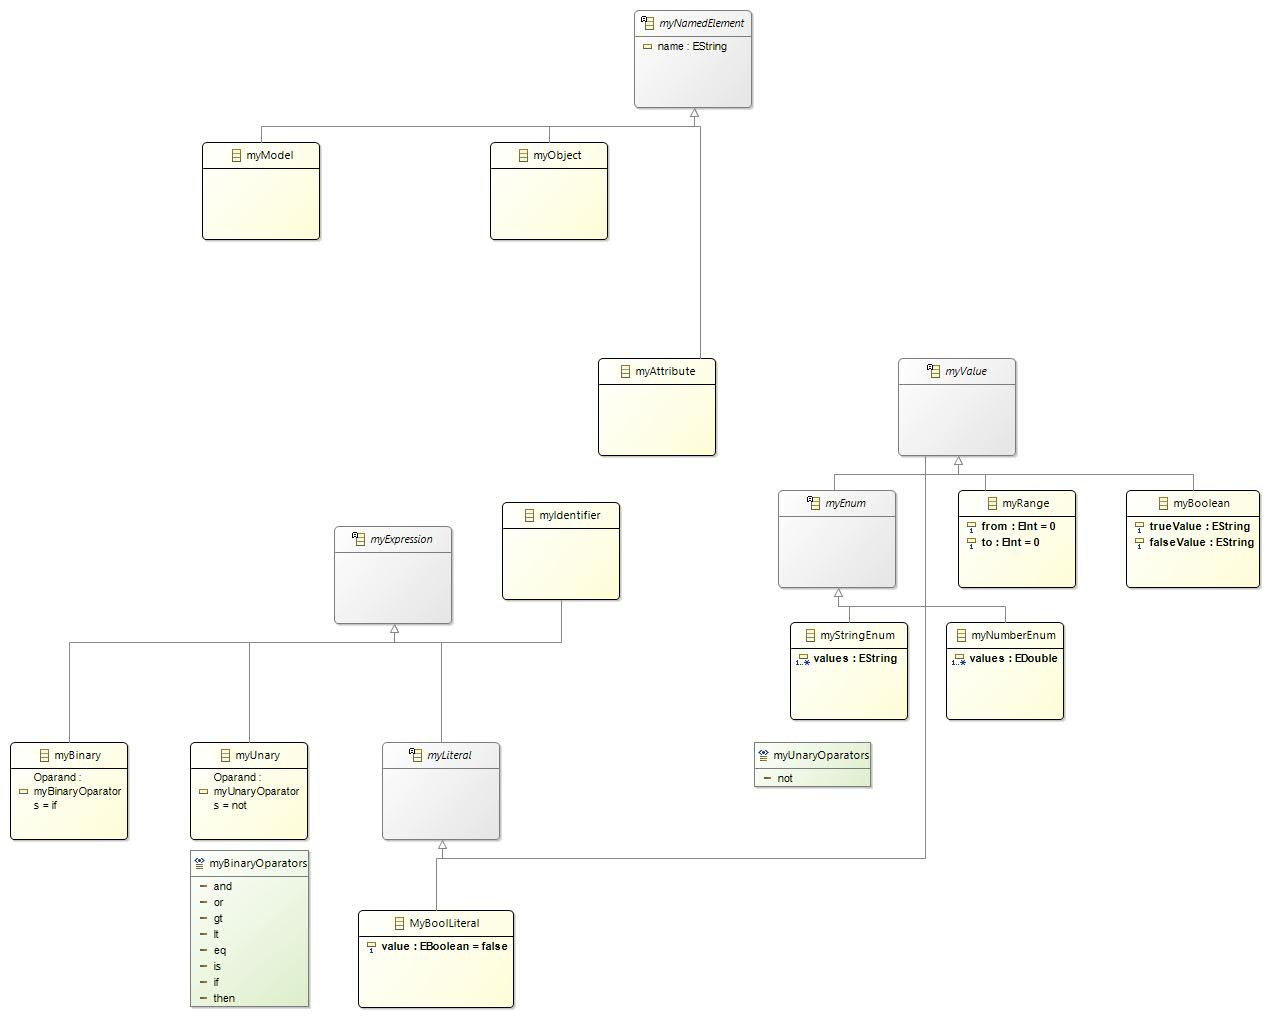
\includegraphics[scale=0.6]{pictures/taxView.jpg}
\caption{Taxonomy View}
\end{figure}

\begin{figure}[H]
\centering
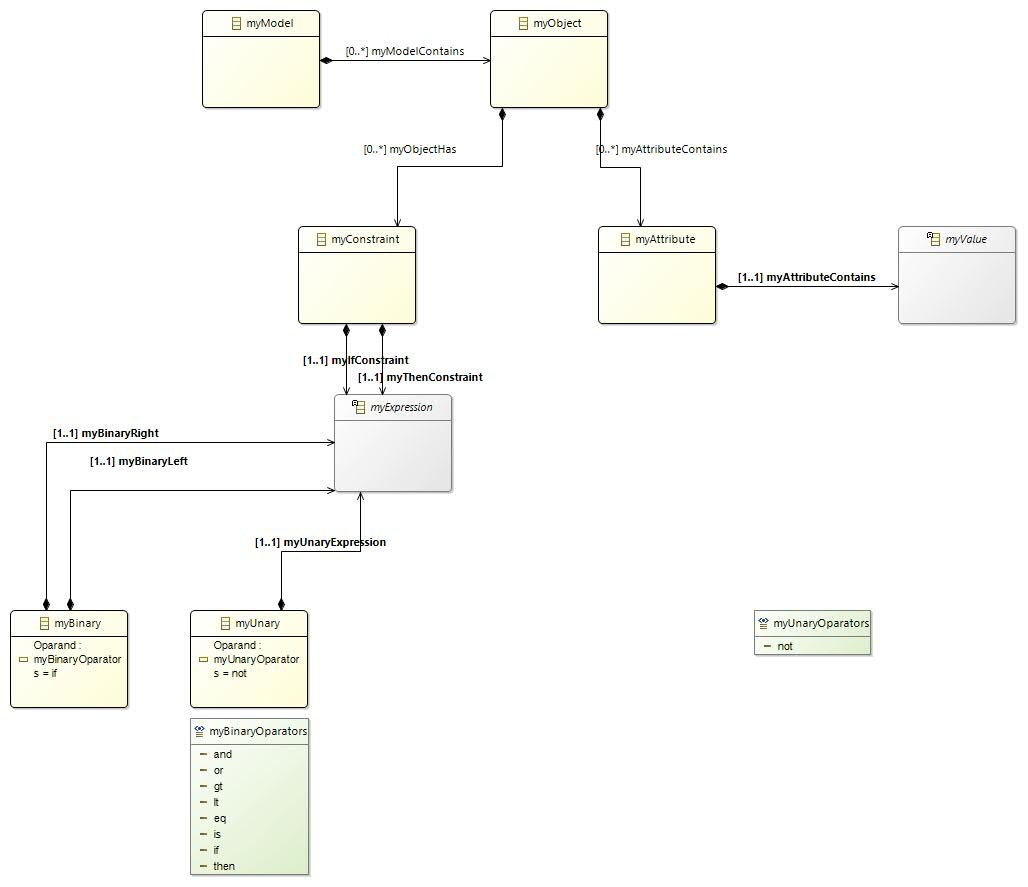
\includegraphics[scale=0.7]{pictures/partView.jpg}
\caption{Partonomy View}
\end{figure}


% 4. Static semantics (constraints, type system). If you have a type checker describe briefly how it works and present the key rules (functions). If you have constraints, includethe entire implementation of the constraints in Xtend with comments explaining the intended semantics in English. No further description is needed.
\section{Static semantics}
\lstinputlisting[language=Java, firstline=35, lastline=244, caption=Static Constraints]{../configproject/xtext/org.xtext.example.smdpdsl/src/org/xtext/example/mydsl/validation/SmdpDslvalidator.xtend}


% 5. Xtext grammar of your language (Concrete Syntax). Just include the .xtext file. You can omit the top imports and other boiler plate, but we want to see all productions. No commentary is expected.
\section{Xtext grammar of your language}
\java{../configproject/xtext/org.xtext.example.smdpdsl/src/org/xtext/example/mydsl/SmdpDsl.xtext}{Xtext Grammar}

% 6. Descriptions of back-ends: the most relevant fragments of your back ends implementation with commentary (max 5 pages in total for both back-ends, not 10 pages). Describe briefly the architecture selected for the two backends (perhaps present an architectural diagram), and show the key aspects of implementation of both back-ends.
\section{Description of back-ends}
We have implemented two code generators, one in html + JavaScript and one in Java. Our HTML consist of a dropdown for each attribute, containing all possible values. After selecting a value for each attribute, the JavaScript checks if it is a valid assignment. The Java code guides the user through each attribute, shows the possible values, and then checks the assignment in the end. Both saves a valid assignment to a txt file.\\

The architecture of both solutions is similar; in each solution, constraints is converted into a set of language specific, valid if statements. With help from a couple of generated helper methods, invalid assignments is removed from the possible values. The assignment is then validated by going through each attribute to check if there are still any values left and if the selected value is still available.\\
The actual conversion of constraints from our domain specific language to either JavaScript or Java is done with a recursive function 'generateIfConstraintString', the function traverses the binary tree and builds a 'if statement'. 

\lstinputlisting[language=Java, firstline=252, lastline=272, caption=generateIfConstraintString method from JavaCodeGenerator.xtend]{../configproject/xtext/org.xtext.example.smdpdsl/src/org/xtext/example/mydsl/generator/JavaCodeGenerator.xtend}

This function uses two helper methods; the first, 'ConvertAttributeName', retrieves the value the user has selected for a given attribute, the other, 'convertOperand', converts our operands from our DSL specific operand type (can, has i.e.) to the language specific equivalent.
For JavaScript, ConvertAttributeName looks like this:

\lstinputlisting[language=Java, firstline=289, lastline=294,caption=ConvertAttributeName method from JavaScriptCodeGenerator.xtend]{../configproject/xtext/org.xtext.example.smdpdsl/src/org/xtext/example/mydsl/generator/JavaScriptCodeGenerator.xtend}

It’s using a HTML5 dom selector to get the selected value and convert it to a double if it’s expected.
The equivalent in the Java, selects the value from a HashMap.

\lstinputlisting[language=Java, firstline=344, lastline=349,caption=ConvertAttributeName method from JavaCodeGenerator.xtend]{../configproject/xtext/org.xtext.example.smdpdsl/src/org/xtext/example/mydsl/generator/JavaCodeGenerator.xtend}

The 'then' part of the if-statement is converted into code that removes invalid values in the recursive method “generateThenConstraintString”. This is again using ”convertOperand” to convert the operand, the generated code is using a hardcoded function to remove the values at runtime.
% SMDP2015\configproject\xtext\org.xtext.example.smdpdsl\src\org\xtext\example\mydsl\generator\ JavaCodeGenerator.xtend (313-334)
\lstinputlisting[language=Java, firstline=313, lastline=334,caption=generateThenConstraintString method from JavaCodeGenerator.xtend]{../configproject/xtext/org.xtext.example.smdpdsl/src/org/xtext/example/mydsl/generator/JavaCodeGenerator.xtend}

\subsection{Back-end |}
\subsection{Back-end ||}

% 7. Test methods and artefacts: Hand in max 1 page description of your test strategy (half a page is recommended) plus max 3 pages of examples of test cases. All in a single PDF file
\section{Test methods and artefacts}
The overall goal for the test phase, have been to make tests covering all possible paths of the implementation, also known as 'path coverage'. This would include testing all possible outcomes in a path.\\ 
This means that the number of tests needed to archive full code coverage is determined by the number of possible paths, in each of the steps from the meta-model until the user frontend. Each path should be tested for both positive and negative testcases.\\

To archive this goal we wish to construct a series of unit-tests within our project using JUnit and Xtend. These tests have been split into three files: \textit{SmdpDslParserTest.xtend}, \textit{SmdpDslGeneratorTest.xtend} and \textit{SmdpDslValidator.xtend}. Each file represents test coverage for one of the three major blocks used in the process from DSL to generated code.\\
The file \textit{SmdpDslParserTest.xtend} contains all tests of the parser, where each test is related to one or more production(s) in the grammar in SmdpDsl.xtext, testing how the types from the concrete syntax is inferred from the model and how the parser behaves when given an unexpected input.\\ 
\textit{SmdpDslValidator.xtend} tests our constraints found in \textit{SmdpDslValidator.xtend}, which is used to validate our DSL. Again, this is testing both intented and unintented input.\\ 
The \textit{SmdpDslGeneratorTest.xtend} file should tests two different aspects of the code. The first is testing that the generated code has the expected layout and syntax and the second being testing that generated code is functioning. \\
In all three files we want to use the same snippets of concrete syntax written in SmdpDsl to act as test caseses.\newline

The above section outlines how the testing part of the project could and should have been made. We have not been able to achieve this fully. One reason being, that we had problems with the way we wanted to test functionality of the generator. A fully implementation of this testing strategy would have lead to a more robust system and it would imply a system with a higher guarantee of expected behavior. \\
Furthermore, all tests have been created towards the end of the project, which isn't optimal in terms of using the test results. Because of this lateness, we have found errors in the project which have not been possible to correct this late in the project.


\newpage

% Examples of parser tests
\lstinputlisting[language=Java, firstline=73, lastline=137,caption=Test examples from SmdpDslParserTest.xtend]{../configproject/xtext/org.xtext.example.smdpdsl.tests/src/org/xtext/example/smdpdsl/tests/SmdpDslParserTest.xtend}

\lstinputlisting[language=Java, firstline=218, lastline=243,caption=Example of negative test from SmdpDslParserTest.xtend]{../configproject/xtext/org.xtext.example.smdpdsl.tests/src/org/xtext/example/smdpdsl/tests/SmdpDslParserTest.xtend}

% Examples of validaton tests
\lstinputlisting[language=Java, firstline=33, lastline=87,caption=Test examples from SmdpDslValidatorTest.xtend]{../configproject/xtext/org.xtext.example.smdpdsl.tests/src/org/xtext/example/smdpdsl/tests/SmdpDslValidatorTest.xtend}

\lstinputlisting[language=Java, firstline=108, lastline=125,caption=Test examples from SmdpDslValidatorTest.xtend]{../configproject/xtext/org.xtext.example.smdpdsl.tests/src/org/xtext/example/smdpdsl/tests/SmdpDslValidatorTest.xtend}

\lstinputlisting[language=Java, firstline=273, lastline=285,caption=Test examples from SmdpDslValidatorTest.xtend]{../configproject/xtext/org.xtext.example.smdpdsl.tests/src/org/xtext/example/smdpdsl/tests/SmdpDslValidatorTest.xtend}



%-------- END --------------------------------------------------------------------------------
\end{document}